\PassOptionsToPackage{utf8}{inputenc}
\documentclass{bioinfo}

\usepackage{makecell}

\usepackage{floatrow}

\usepackage{comment}

\usepackage{siunitx}

% singlelinecheck=false puts subcaptions on the left
\usepackage[singlelinecheck=false]{subcaption}

\usepackage[usenames,dvipsnames]{xcolor}

\usepackage{amsthm}
\theoremstyle{definition}
\newtheorem{definition}{Definition}[section]
\newtheorem{theorem}{Theorem}[section]
\newtheorem{corollary}{Corollary}[theorem]
\newtheorem{lemma}[theorem]{Lemma}

\usepackage{algorithm2e}
\SetKwRepeat{Do}{do}{while}%

% we squeeze our figures even more together
\captionsetup{belowskip=-2pt}

\SetAlgoLined
\SetKwProg{MyStruct}{Struct}{ contains}{end}

\newcommand{\vocab}{\textbf}
\newcommand{\red}[1]{{\textcolor{Red}{#1}}}
\newcommand{\FIXME}[1]{\red{[FIXME: #1]}}

\usepackage{orcidlink}
\hypersetup{hidelinks}


\def\labelitemi{--}

\copyrightyear{2022} \pubyear{XXXX}

\access{Advance Access Publication Date: Day Month Year}
\appnotes{Genome Analysis}

\begin{document}
\firstpage{1}

\subtitle{Genome Analysis}

\title[Unbiased pangenome graphs]{Unbiased pangenome graphs}
\author[Garrison \textit{et~al}.]{
Erik~Garrison\,$^{\orcidlink{0000-0003-3821-631X}\text{\sfb 1}*}$,
Andrea~Guarracino\,$^{\orcidlink{0000-0001-9744-131X}\text{\sfb 2}}$
}

\address{
$^{\text{\sf 1}}$University of Tennessee Health Science Center, Memphis, TN, USA \\
$^{\text{\sf 2}}$Genomics Research Centre, Human Technopole, Milan, Italy
}

\corresp{
$^\ast$To whom correspondence should be addressed. \\
% $^\dagger$Contributed equally.\
}

\history{Received on XXXXX; revised on XXXXX; accepted on XXXXX}

\editor{Associate Editor: XXXXXXX}

\abstract{
\textbf{Motivation:}
Pangenome variation graphs model the mutual alignment of collections of DNA sequences.
A set of pairwise alignments implies a variation graph, but there are no scalable methods to generate such a graph from these alignments.
Existing related approaches depend on a single reference, a specific ordering of genomes, or a \textit{de Bruijn} model based on a fixed $k$-mer length. %, and may not describe the base-level alignment of genomes into the pangenome.
A scalable, self-contained method to build pangenome graphs without such limitations would be a key step in pangenome construction and manipulation pipelines. \\
\textbf{Results:}
We design the \textit{seqwish} algorithm, which builds a variation graph from a set of sequences and alignments between them.
We first transform the alignment set into an implicit interval tree.
To build up the variation graph, we query this tree-based representation of the alignments to reduce transitive matches into single DNA segments in a sequence graph.
By recording the mapping from input sequence to output graph, we can trace the original paths through this graph, yielding a pangenome variation graph.
We present an implementation that operates in external memory, using disk-backed data structures and lock-free parallel methods to drive the core graph induction step.
We demonstrate that our method scales to very large graph induction problems by applying it to build pangenome graphs for several species. \\
\textbf{Availability:}
\textit{seqwish} is published as free software under the MIT open source license.
Source code and documentation are available at \url{https://github.com/ekg/seqwish}.
\textit{seqwish} can be installed via Bioconda \url{https://bioconda.github.io/recipes/seqwish/README.html} or GNU Guix \url{https://github.com/ekg/guix-genomics/blob/master/seqwish.scm}. \\
\textbf{Contact:} \href{egarris5@uthsc.edu}{egarris5@uthsc.edu} \\
%\textbf{Supplementary information:} Supplementary data are available at \textit{Bioinformatics} online.
}

\maketitle


\section{Introduction}
\label{sec:introduction}
A pangenome models the full genomic information of a species or clade \citep{Medini_2005,Sherman_2020}.
In contrast to reference-based approaches that relate sequences to a particular reference genome, methods that use pangenome reference systems attempt to model the mutual relationship between all represented genomes \citep{cpang2018}.
%These models encode the mutual relationships between all the genomes represented, in contrast to reference-based approaches which relate sequences only to a particular ``reference'' genome.
%In principle, pangenome graphs can allow for a great reduction in reference bias, allowing any part of a pangenome to be considered in biological studies. %, and may provide a simpler representation of structurally-variable regions.
Many approaches model the pangenome alignment as a \textit{pangenome graph} \citep{Garrison_2018,Yokoyama2019,Hickey:2020}.
A pangenome graph encodes DNA sequences as walks through an underlying language encoded in a sequence graph \citep{Hein_1989}.
In a pangenome graph, variation can be understood in the context of any part of any included genome  \citep{Eizenga_2020}.
This lets us avoid the problem of reference bias, which can be understood as the limitation of analyses to genome sequences that are similar to a chosen reference genome.
%Reference bias distorts an inferred genome to appear more similar to the reference genome than it actually is.

An unbiased pangenome graph would represent the alignment of all included genomes to all others.
Existing methods approximate this relationship by progressive alignment to a graph initially based on a reference genome \citep{Li:2020}, through a global structuring of the genome relationships in a neighbor joining phylogenetic tree \citep{Armstrong:2020}, or via creation of a \textit{de Bruijn} graph based on a fixed $k$-mer length \citep{Minkin_2016,Yu_2021}.
These methods limit computational costs by reducing the number of pairwise comparisons, but in turn their results depend on input genome order, selected reference, guide-tree topology, or $k$-mer length.

We consider the problem of building a pangenome graph without these potential sources of bias.
Such a graph would be an ideal system to represent variation between two or more high-quality genomes.
Given the rapid development of complete genome assemblies for humans and other vertebrates \citep{Rhie_2021,Nurk_2021}, we need a practical approach that can achieve this for tens to thousands of genomes on commodity hardware.
Here, we present \textit{seqwish}, an algorithm for the generation of a pangenome graph from pairwise alignments.
%It transforms a collection of sequences and their alignments into a series of intermediate representations that support the computation of an equivalent pangenome graph.
Our solution is simple, but experiments on diverse sequence collections demonstrate that it easily scales to large pangenome building problems.
%It is also, by focus on the key graph induction step, a simple component.

%Our solution is simple, but flexible, and we demonstrate its scalability to pangenome construction problems in diverse genomes.

%As the diffic for model organisms \citep{Rhie_2021,Nurk_2021}
%, we consider the need to efficiently construct \textit{unbiased} pangenome graphs based on symmetric relationships among sequences.

%Furthermore, Minigraph does not provide base-level information, limiting the analysis to only large structural variation.
%Although a reference-guided approach is pragmatic when we only have a single reference genome, recent advances in sequencing and assembly are driving the generation of many reference-quality assemblies in humans and other species \citep{Nurk_2021}.

%A class of methods to represent pangenomes involves the \textit{sequence graph} \citep{Hein_1989}, where identical segments of different genomes collapse into a single representative segment (often node) in the graph.
%In \textit{node-labeled} sequence graphs, nodes indicate DNA sequences, with edges connecting the nodes that are concatenated in the sequences represented in the graph.
%A \textit{bidirected} sequence graph represents both strands of DNA.
%On this model, variation graphs add the concept of \textit{path} to embed linear sequences (e.g., genomes or haplotypes) into the graph \citep{Garrison_2018}.
%Paths provide a stable coordinate system, allowing graph annotations and interoperability between different graphs.

%A pangenome graph is a sequence model that encodes the mutual alignment of many genomes \citep{Eizenga_2020}.

%Motivated by the need to generate ``multi-reference'' pangenome graphs, we develop \textit{seqwish}, an algorithm that allows us to build pangenome graphs in the form of variation graphs directly from a collection of sequences and pairwise alignments between them.
%Here, we formally describe the algorithm, evaluate its basic combinatorial bounds and costs, and present applications of the method to pangenome building problems in a variety of species.

%Our approach is both highly generic and scalable.
%Not only is our approach highly generic,but it also efficiently scales to both large and complex pangenomes.
%with \textit{any} collection of alignments and sequences, 


%Given recent advances in genome sequencing and assembly, we expect that soon, many species will have multiple reference-quality genomes.
%To build a pangenome model from such genomes that is truly unbiased, we need an approach to build a multi-reference 
%Motivated by the current availability of two reference-quality human genome assemblies 
%The inability to build pangenome graphs from 

\section{Algorithm}
\label{sec:algorithm}

In this section, we provide a formal definition of variation graph induction.
We then examine the bounds of a na\"{i}ve implementation of this algorithm.
Finally, we propose compression and partitioning techniques to reduce the space and working memory complexity of the induction process by a large constant factor modulated by the degree of sequence divergence in the input pangenome.
This yields a practical algorithm for variation graph induction that can scale to the largest available pangenomes.

\subsection{Variation graph induction}

\begin{definition}
\label{def:vg}
Variation graphs are a common formalism to encode pangenome graphs \citep{Garrison_2019_thesis}.
In the variation graph $\mathcal{V} = (\mathcal{N}, \mathcal{E}, \mathcal{P})$, nodes $\mathcal{N} = n_1\ldots n_{|\mathcal{N}|}$ contain sequences of DNA.
Each node $n_i$ has a unique identifier $i$ and an implicit reverse complement $\bar{n_i}$.
A node strand $s$ corresponds to one node orientation.
Edges $\mathcal{E} = e_1\ldots e_{|\mathcal{E}|}$ connect ordered pairs of node strands ($e_i = ( s_a, s_b )$), encoding the base topology of the graph.
Paths $\mathcal{P} = p_1\ldots p_{|\mathcal{P}|}$ describe walks over node strands ($p_i = s_1 \ldots s_{|p_i|}$), representing the collection of genomes embedded in the graph.
\end{definition}

\begin{theorem}
A variation graph represents pairwise alignments between its embedded paths.
\end{theorem}

\begin{proof}
By definition \ref{def:vg}, two paths have identical subsequences where they walk (or step) through the same series of oriented nodes (e.g. $s_1 s_2 s_3$).
An identical set of path steps is thus equivalent to a sequence match.
Pairwise alignments are by definition collections of character-level matches between sequences.
The variation graph thus models a set of pairwise alignments between paths in $\mathcal{P}$.
\end{proof}

\begin{theorem}
\label{thm:seqwish}
%\textit{seqwish}:
We can build a variation graph from sequences and pairwise alignments.
The resulting variation graph fully embeds both the sequences and all pairwise relationships in the input.
\end{theorem}

This follows from \ref{def:vg}.
Our input $Q = S \vee \bar{S}$ is a set of $N$ DNA sequences $S = g_1 \ldots g_N$ and their reverse complements $\bar{S} = \bar{g_1} \ldots \bar{g_N}$.
%Assume that $i$ and $j$ are coordinates in $Q$.
A match $m = (i, j)$ asserts the aligned equivalence of two characters in sequences in $Q$.
%$\forall_{(i, j) : j = |g| - i} g[i] = \bar{g}[j]$.
Pairwise alignments between sequences in $Q$ are a set of matches $A = \{ m_1 \ldots m_{|A|} \}$.
By standard definition, each sequence matches its own reverse complement, that is $g[i] = \bar{g}[j]$ for all $j = |g| - i$, and we assume these matches are included in $A$.
%A match $m$ can be understood as a component in a binary relation.
The transitive closure of a match, $m^+ = \{ i \ldots j \}$, is a set of characters in $Q$ that are transitively linked together by other matches.
By definition of $m$, each $m^+$ implies a single, identical character $c(m^+)$.

We build a graph $\mathcal{V}$ inductively.
We take the first match in $A$, $m_1$, and execute a union-find operation to obtain $m_1^+$.
We add the character of the match $c(m_1^+)$ as a node $n_1$ in $\mathcal{V}$, and record the mapping from $m_1^+ \to n_1$.
To induce the graph, we take the next unused match in $A : m_i \notin \forall_{j < i} m_j^+$, obtain $m_i^+$, and add $c(m_i^+)$ to $\mathcal{V}$.
To allow the annotation of paths, we record the set of characters in $Q$ that match to a given node in $\mathcal{V}$ in mapping $Z = Q \to \mathcal{N} = m_1 \ldots m_{|\mathcal{N}|}$.
We continue until all matches have been used.
Finally, we establish paths ($\mathcal{P}$) by walking them in $\mathcal{V}$ using $Z$, and record edges ($\mathcal{E}$) where nodes occur successively in paths.

\begin{proof}
After the first step of induction, the graph represents all pairwise matches in $m_1^+$.
Each subsequent step includes progressively more of $A$, until at completion, all pairwise relationships are accounted for in $V$.
%All characters in $S$ have been accounted for in $V$, and we can make this mapping explicit by tracing $S$ through the
%The paths of the variation graph are equivalent to input sequences, and the path relationship within the graph is defined by their alignments.
\end{proof}

The set of alignments represented by a variation graph is strictly larger than the set of alignments used to induce it.
The graph must contain at least the set of alignments given in input.
It may also contain new implied pairwise relationships that arise due to transitive match relationships, as shown in Figure \ref{fig:induction} for closures 1 and 6.
However, by definition of $\mathcal{V}$, it cannot contain \textit{less} match information than represented in the set of matches ($A$).

\vspace{-1em}
\begin{figure}[ht!]
%  \centering
    \floatbox[{\capbeside\thisfloatsetup{capbesideposition={left,top},capbesidewidth=0.45\linewidth}}]{figure}[\FBwidth]
    {\caption{\FIXME{put high-resolution image} Building variation graphs from alignment graphs. Top: an alignment graph between a set of sequences,
        showing alignment edges in grey and precedence (path) edges in colors associated with each path. Bottom: the variation graph
        resulting from the application of the transitive closure process in \textit{seqwish}, where aligned segments have been
        compressed into a single node.
    }\label{fig:from_alignment_to_variation_graph}}
    %{
\includegraphics[width=\linewidth]{fig/OUP_First_SBk_Bot_8401}} %\includegraphics[width=5cm]{name}}
    %\caption{Performance evaluation of \textit{odgi build} when translating a 90-haplotype graph of human chromosome 6 into ODGI's native format.}

\end{figure}
\vspace{-1em}

\subsection{Induction algorithm sketch}

%Although the space bounds alone indicate that this approach is infeasible, we can also consider its time complexity.
%First, we must enable random access to match elements in $A$.
%Assuming that $A$ contains pairs of characters in $Q$, then we can sort it
For the sake of time and space complexity analysis, we consider a simple algorithm to implement the induction process.
The induction depends on our ability to compute transitive closures of matches $m^+$.
If $A$ is sorted, we can find the matches of a given character in $Q$ using binary search, which allows us to compute $m^+$ for each character.
We do so non-redundantly by marking each used character in $Q$ in an auxiliary data structure $\mathcal{X}$, which could be encoded as a bitvector of length $|Q|$.
As we compute the transitive closures, we emit both the nodes (single characters) of the graph $\mathcal{N}$ and the sequence-to-graph mapping $Z$, which, like $A$, consists of match pairs, but rather than mapping $Q \to Q$, maps $Q \to \mathcal{N}$.
As with $A$, we can sort $Z$ to obtain random access via binary search.
Finally, we derive elements in $\mathcal{P}$ by iterating through the characters of $Q$ and looking up their mapping in $Z$ using binary search.
The edge set $\mathcal{E}$ are the unique pairs of steps found in $\mathcal{P}$, and can be computed by sorting pairs of steps in $\mathcal{P}$.

%We construct an index $A_{idx}$ which allows us to query the matches of each character in $Q$.

\subsection{Na\"{i}ve algorithm bounds}
\label{sec:bounds}

The inductive proof of theorem \ref{thm:seqwish} demonstrates how to build a variation graph from sequences and their pairwise alignments.
However, a na\"{i}ve algorithm based on this model would require a very large amount of space.
Take $\mathcal{Q} = |S|$.
Although our identifier space $\mathcal{Q}$ must include all of $Q$, in practice, we only store $S$, as $\bar{S}$ can be trivially computed.
Assume an all-to-all alignment of $N$ sequences in $A$ as input, and that all sequences are approximately identical, so that the induced variation graph has $\mathcal{Q}/N$ nodes.
The induction must maintain reference to all characters in all input sequences $O(\mathcal{Q})$, all character-to-character matches $O(|A|) \approx O(\mathcal{Q}N^2)$, the mapping of $Q$ into the graph $O(|Z|) \approx O(\mathcal{Q})$, the nodes of the graph $O(|\mathcal{N}|) \approx O(\mathcal{Q}/N)$, the size of the edge set $O(|\mathcal{E}|) \approx O(\mathcal{Q})$, and the set of paths $O(|\mathcal{P}|) \approx O(\mathcal{Q})$.
We also maintain the bitvector $\mathcal{X}$ to mark seen characters of $Q$ during graph induction, which requires $O(\mathcal{Q})$ bits, equivalent to $O(\mathcal{Q} / \log_2\mathcal{Q})$ integer identifiers.
In total, na\"{i}ve theorem \ref{thm:seqwish}-based induction would require approximately $O(\mathcal{Q}(N^2 + 1/N + 1/log_2{Q} + 4))$ space.

Assuming that we want to build a graph of 100 haploid human genomes of $\num{3e9}$ bp, where $N=100$ and $\mathcal{Q} \approx \num{e11}$, we might expect to use $\approx \num{e15}$ identifiers to store the full model.
Such a design is almost infeasible for inputs larger than a handful of genomes.
For instance, we would need $\approx \num{3e12}$ identifiers for just 5 human genomes.
Although it is feasible to compute such a graph using external memory, the approximately 200-fold increase in space relative to the input renders this clearly impractical.

Considering the time complexity of induction, we anticipate $O(|A|\log|A|)$ time to sort the match set and $O(\mathcal{N} \log |A|)$ to query it and compute our $\mathcal{N}$ transitive closures.
Computing the variation graph paths $\mathcal{P}$ involves converting sequences in $S$ to walks through $\mathcal{N}$.
We first sort the sequence-to-graph mapping array $Z$ in $O(\mathcal{Q} \log \mathcal{Q})$ operations, and then compute $\mathcal{P}$ in $O(\mathcal{Q})$ queries which each cost $O(\log \mathcal{Q})$.
To obtain unique edges and generate $\mathcal{E}$, we must build and sort an array of $O(2\mathcal{P})$, and then iterate through it for $O(2\mathcal{P} \log 2\mathcal{P} + 2\mathcal{P})$ operations.
In sum, we would expect to require $O(|A|\log|A| + \mathcal{N} \log |A| + 2(\mathcal{Q} \log \mathcal{Q}) + 2(\mathcal{P} \log 2\mathcal{P} + \mathcal{P}))$.
Using our approximate relationships to $\mathcal{Q}$ given previously and simplifying, we arrive at $O[\mathcal{Q}(2N^2 \log N / \log \mathcal{Q} + (1/N + 4)\log \mathcal{Q} + 2 + log(4))]$.

Due to our dependence on sorting, and the logarithmic-time cost of queries, growth in $\mathcal{Q}$ drives $\Omega(\mathcal{Q} \log \mathcal{Q})$ growth in overall complexity.
As $N$ grows, both time and space complexity are dominated by the number of alignments, which in the case of our example is $O(N^2)$.
For large numbers of highly-similar genomes, we may not require all pairs of alignments to build a graph that contains all pairwise alignments.
Various approaches could be used to reduce the size of $A$ without disrupting the induced graph.
We leave these to later work.

%In practice, it is likely that this can be considerably reduced with minimal effect , particularly for
%In practice, for large numbers of highly similar genomes, it a true all-pairs alignment may be unnecessary, but the construction of a graph that represents all-pairwise alignments 
%In practical applications, it is unlikely that we will need a true all-pairs alignments for highly similar genomes, and this could be considerably reduced with heuristics that

%we likely  a true all pairs alignment, but limiting this requires heuristic schemes to generate a set of alignments that does not cause any match transitive closures to be partitioned. This topic lies outside the scope of this work.

%$O[(\mathcal{Q}/N + 5\mathcal{Q}) \log \mathcal{Q} + \mathcal{Q}(2 + log(4))]$.
%$O(\mathcal{Q} \log \mathcal{Q} + \mathcal{Q}/N \log \mathcal{Q} + 2(\mathcal{Q} \log \mathcal{Q}) + 2(\mathcal{Q} \log 2\mathcal{Q} + \mathcal{Q}))$.

%(note that this would 
%To enable random access to match elements between $A$
%Continuing our assumed graph context, with quasi-identical genomes and an all-to-all alignment between them, we can compute each match closure operation 
%The cost of each transitive closure operation should be 

\subsection{Match compression}
\label{sec:matchcompression}

As the bounds analysis shows, space requirements make it impractical to apply a trivial version of theorem \ref{thm:seqwish} to generate a large pangenome graph.
Therefore, we need a compression approach that exploits redundancy in the input genomes to reduce the costs of the algorithm.
When working with large numbers of genomes, alignments dominate the computational costs.
A simple technique is to generalize matches $m = (i, j)$, which are between individual characters, to \textit{range}-matches over pairs of ranges of characters in $Q$.
For highly-similar sequences, our expectation is that exact matches will occur in long runs.
If the average pairwise diversity of sequences in our input is $1/k$, we expect exact matches to be around $k$ characters long.
By encoding matches as pairs of ranges of characters, $r = (a, b) : a, b = (i, j) : i, j \in Q$, we can obtain a $\approx$ $k$-fold compression of $A$, yielding the range-match array $\mathcal{A}$.

If sorted, $\mathcal{A}$ can be treated as an \textit{implicit interval tree} \citep{Li_bedtk_2020}, which allows queries of containment and overlap in $O(\log |\mathcal{A}|)$ time.
This compression requires trivial changes to our graph induction model.
To obtain our match transitive closures ($m^+$), we query $\mathcal{A}$ for the range of a single character in $Q$, computing the character-level transitive relationships from the relative offsets of the ranges in $\mathcal{A}$.
Match compression thus reduces our alignment storage memory bounds by a factor of $k$ without affecting our time complexity bounds.

The same encoding can be used to replace the sequence-to-graph mapping $Z$, yielding $\mathcal{Z}$.
Rather than pairs of characters in $Q$ and $\mathcal{N}$, we record runs of matches between them as range matches.
Although in expectation the length of these matches should be strictly less than $k$, due to the interruption of the graph by variation between genomes, this still allows us to reduce the size of $Z$ using runs of matches between $Q$ and $\mathcal{N}$.
Additionally, we store the inverse of $\mathcal{Z}$, which maps ranges from $\mathcal{N} \to Q$, as $\bar{\mathcal{Z}}$.
We use $\mathcal{Z}$ to compact non-branching regions of $\mathcal{V}$ into single nodes, and $\bar{\mathcal{Z}}$ to accelerate our calculation of links in the graph.

%We can save $\approx k$ match pairs per recorded range 
%a pair of ranges $r = [(a_0, a_1), (b_0, b_1)]$ in $Q$ requires twice the space, but we expect it to 

%The dominance of alignments in our space costs make
%In practice, the cost of

%We render this 

\begin{algorithm}[hb!]

\SetKwFunction{MakeMatchIITree}{MakeMatchIITree}
\SetKwFunction{MakeIITree}{MakeIITree}
\SetKwFunction{GetTransitiveMatches}{GetTransitiveMatches}
\SetKwFunction{AddNode}{AddNode}
\SetKwFunction{BitVector}{BitVector}
\SetKwFunction{ExtendRanges}{ExtendRanges}
\SetKwFunction{FirstOverlap}{FirstOverlap}
\SetKwFunction{Overlaps}{Overlaps}
\SetKwFunction{NodeMatching}{NodeMatching}
\SetKwInOut{Input}{input}\SetKwInOut{Output}{output}
\Input{sequences $S$ and their alignment $A$}
\Output{variation graph $\mathcal{V} = (\mathcal{N}, \mathcal{E}, \mathcal{P})$}
$\mathcal{A}\gets$ \MakeMatchIITree{$A$} \tcp{alignment matches}
$\mathcal{N}\gets \emptyset$ \tcp{vector containing the set of nodes}
$\mathcal{X}\gets$ \BitVector{$0, |S|$} \tcp{seen characters of $S$}
\tcp{for each character in the input}
\For{$i\leftarrow 1$ \KwTo $|S|$}{
  \tcp{this character is not yet in $\mathcal{V}$}
  \If{$\mathcal{X}[i] = 0$}
  {
    \tcp{characters in $S$ matched to $i$}
    $m^+_i$ $\gets$ \GetTransitiveMatches{$\mathcal{A}$, $i$} \\
    $\mathcal{N} \gets $ \AddNode{$\mathcal{N}$, $c(m^+_i)$} \tcp{new node in $\mathcal{V}$}
    $j \gets |\mathcal{N}|$ \tcp{the node id or rank in $\mathcal{V}$}
    \For{$z \in m^+_i$}{
     $X[z] \gets 1$  \tcp{mark seen character}
     $\mathcal{Z} \gets $ \ExtendRanges{$\mathcal{Z}$, z, j} \tcp{query$\to$graph}
     $\bar{\mathcal{Z}} \gets $ \ExtendRanges{$\bar{\mathcal{Z}}$, j, z} \tcp{graph$\to$query}
    }
  }
}
\tcp{set up our $S \to \mathcal{N}$ mappings}
$\mathcal{Z} \gets $ \MakeIITree{$\mathcal{Z}$};
$\mathcal{\bar{Z}} \gets $ \MakeIITree{$\mathcal{\bar{Z}}$} \\
\tcp{compact nodes in $\mathcal{N}$ yielding $\mathcal{N}'$}
$\mathcal{N}' \gets \emptyset$ ; $l \gets \emptyset$ ; $b \gets 0$ ; $\mathcal{B}\gets$ \BitVector{$0, |\mathcal{N}|$} \\
%$l \gets \emptset$ \tcp{compacted nodes and }
\For{$i\leftarrow 1$ \KwTo $|\mathcal{N}|$}{
  $m \gets $ \Overlaps{$\mathcal{\bar{Z}}$, $i$} \\
  \If{$m \ne l$}{
  $B[i] = 1$ \tcp{record a node boundary}
  $\mathcal{N}' \gets $ \AddNode{$\mathcal{N}'$, $\mathcal{N}[b\ldots i]$} \\
  $b \gets i$ \tcp{record last node boundary}
  }
  $l \gets m$ \tcp{our last set of matching ranges}
}
$\mathcal{P}\gets \emptyset$;
$\mathcal{E}\gets \emptyset$ \tcp{paths and edges}
$q \gets 1$ \tcp{for each sequence in the input}
\For{$i\leftarrow 1$ \KwTo $N$}{
  $p_i \gets \emptyset$ ;
  $j \gets q$ ;
  $y \gets 0$ \\
  \Do{$j < q + |g_i|$}{
    \tcp{extend our path with the next step}
    $(a, b) \gets$ \FirstOverlap{$\mathcal{Z}, j$} \\
    $x \gets$ \NodeMatching{$\mathcal{N}'$, $\mathcal{B}$, $(a, b)$} \\
    $p_i \gets p_i + x$ \tcp{extend the path}
    $j \gets j + (b - a)$ \tcp{increment offset in $S$}
    $\mathcal{E} \gets \mathcal{E} \cup \{(y, x)\}$ \tcp{add to our edge set}
    $y \gets x$ \tcp{record last step}
  }
  $q \gets j$ \tcp{increment our pointer in $S$}
}
\Return{$\mathcal{V} \gets (\mathcal{N}', \mathcal{E}, \mathcal{P})$} \\
\vspace{2mm}
\caption{The \textit{seqwish} graph induction algorithm.
  For the sake of simplicity, we omit the details of several query algorithms that interact with the input alignments, the transitive match closure, implicit interval tree construction and query, node generation, and bitvector rank queries used in node compaction.
  Similarly, we omit the details of the input partitioning that we use to reduce maximum resident memory requirements.
}
\label{alg:seqwish}
\end{algorithm}


\subsection{Node compaction}

For simplicity, we have thus far presented a character-level model of variation graph induction.
However, range (or run) compression can also reduce the representation size of the graph.
Rather than recording an identifier for each character in a sequence graph, it is useful to compact characters that form trivial linear components in the graph into single nodes.
Broadly, the size of nodes will be bounded by the average distance between variants, which, for pangenomes built from \textasciitilde100 individuals of the same species, often provides a great reduction in the total number of nodes (and thus identifiers) required for $\mathcal{V}$ and its components.

To compact $\mathcal{V}$, we traverse $Q$, finding each entry in $\mathcal{Z}$ in turn, recording its start and end in $\mathcal{N}$, which can be understood as a character vector or string containing all the sequence in the nodes of $\mathcal{V}$.
%in a ``graph vector'' $\mathcal{G} = n_1,n_2 \ldots n_{|\mathcal{N}|}$ containing the ordered characters of the graph.
%Any position in $\mathcal{G}$ so marked must be the start or end of a node.
We subsequently use these markings to subdivide $\mathcal{N}$ into a compacted version $\mathcal{N}'$ where compacted node boundaries are marked in a auxiliary bitvector $\mathcal{B} : |\mathcal{B}| = |\mathcal{N}|$ where the first character in each compacted node is marked by a $1$ and other characters are marked $0$.
$\mathcal{B}$ allows us to compute compacted node ids using efficient rank operations \citep{Gog_2014}.
%such that $\forall_{i \in 1 \ldots |\mathcal{N}'|} |n_i| \ge 1$.
%In Algorithm \ref{alg:seqwish} we provide a detailed description of the graph induction algorithm.

%\FIXME{For reasons of computational efficiency, node identifiers are numeric.}

\subsection{Induction partitioning}
\label{sec:partitioning}

Although match compression provides an approximate factor $k$ improvement in memory bounds for key data structures used in the induction, the approach we present in section \ref{sec:matchcompression} requires working memory in the order of the set of transitive match closures in the graph.
A simple approach to reduce this bound is to divide the induction problem into smaller pieces.
We do so by computing the graph induction for a collection of initial characters in $Q$.
%We induce the related graph for each partition, appending the induction results to the appropriate data structures.
In each partition, we apply a lock-free parallel union-find algorithm to derive the match closures \citep{anderson1991wait}, appending results to appropriate data structures.
This partitioning can introduce boundary effects which change the contents of $\mathcal{Z}$ and $\bar{\mathcal{Z}}$ by splitting ranges at the boundaries of our partitions.
However, while this will affect the compressed node definition $\mathcal{N}'$, it does not affect $\mathcal{N}$, and it can be corrected via a post-processing step to sort and compact the id space.
%Partitioning reduces the working memory limits to be in the order of the size of the largest transitive match closure found in the input.


\section{Implementation}

We have presented a complete model for variation graph induction from sequences and their pairwise alignments (Algorithm \ref{alg:seqwish}).
Here, we describe our specific implementation of this algorithm: \textit{seqwish}.
In general, our approach uses external memory to elaborate the graph, taking advantage of the availability of low-latency storage media, like solid-state drives (SSDs), to maximize the performance of this approach.

\subsection{Input and output processing}

%A practical implementation introduces a new set of problems related to input and output. % that we have not yet introduced.
Our implementation reads standard data formats, FASTA or FASTQ for the input sequences, and PAF \citep{Li_2018} for pairwise alignments.
It writes the graph in standard Graphical Fragment Assembly (GFA) format \citep{GFA}.

In PAF, the input set of alignments is not directly expressed in terms of matches between specific characters in $Q$.
Rather, each record lists the name of the aligned pair of query and target sequences and offsets in each.
To efficiently process the input PAF, we thus need to build a sequence index that allows us to generate $\mathcal{A}$.
In particular, we build a compressed suffix array (CSA) \citep{Sadakane_2000} over sequence names, that we call \textit{seqidx}, and provide auxiliary supporting data structures that allow us to map between our input and the abstract concatenation of all input sequences and their reverse complements ($Q$).
We often build graphs from very large collections of sequences, such as raw sequencing reads or contigs from many thousands of samples.
This \textit{seqidx} avoids the overheads associated with a hash table on string names of input sequences.
To enable highly-efficient random access, we cache the input sequences in a disk-backed version of $Q$, into which our queries of sequence name and offset point.
This trades time that might be spent accessing a compressed representation of the input for space in external memory.

For output in GFA, we iterate over nodes in $\mathcal{N}'$, writing each as a node record.
Edges are similarly produced from the disk-backed multiset representing $\mathcal{E}$.
The most computationally expensive part of graph emission is the rendering of the input sequences $S$ as paths $\mathcal{P}$ through the graph.
For each input sequence in the \textit{seqidx}, we walk through the offsets in $S$ contained in the sequence and look up their mapping into $\mathcal{N}'$ using $\mathcal{Z}$.
Range compression allows us to complete one lookup per range.
By definition, each character in $S$ is covered by only one range in $\mathcal{Z}$.
We can thus iterate through the ranges in $\mathcal{Z}$ without considering each character.
Following the GFA format, we are able to independently generate $\mathcal{P}$, as each path is represented on a separate record in the GFA.

\subsection{Key disk-backed data structures}

In our implementation, we rely on several basic external memory kernels.
To reduce working memory requirements to an absolute minimum, we use a disk-backed version of the implicit interval tree that memory-maps the sorted array of intervals \citep{mmmulti}.
Indexing the implicit interval tree requires a sorting step which dominates the runtime of our algorithm.
We adapt the current best-performing in-place parallel sorting algorithm, In-place Parallel Super Scalar Samplesort (IPS$^4$o), to work on a disk-backed, memory-mapped array \citep{axtmann2017}.
This allows us work with $\mathcal{A}$, $\mathcal{Z}$, and $\bar{\mathcal{Z}}$ in external memory.
By storing pairs of numerical identifiers in the backing array, we are able to generate a disk-backed multiset model which we use to compute the unique set of edges $\mathcal{E}$ in terms of offsets in $\mathcal{N}$.
The graph sequence vector $\mathcal{N}$ is simply written by appending characters to a file.
We mark nodes to generate $\mathcal{N}'$ using a bitvector kept in main memory, over which we subsequently generate a rank/select dictionary \citep{Gog_2014} for support of the final emission of the graph $\mathcal{V}$.

\subsection{Short match filter}
\label{sec:filter}

Building a graph from an all-to-all alignment does not guarantee that the local structure of the graph is easy to understand.
The all-to-all alignment is not coordinated, with each mapping aligned in isolation, and in consequence it fails to resolve the indel alignment normalization problem \citep{Mose_2019}.
This ambiguity can introduce deeply looping structures in the graph which collapse polymorphic microsatellites and other short VNTRs into very small numbers of nodes with very complex local topologies.
Such motifs can cause problems with downstream analysis.
We find that ambiguity about the arrangement of very short matches tends to drive complex local structures in the graph.

We mitigate this issue with a simple filter, \textit{seqwish -k}, which simply ignores exact matches that are shorter than $k$ characters.
This filter necessarily increases the size of the induced graph.
But, it also replaces complex motifs shorter than $k$ with single bubbles.
In doing so, it also removes short, expensive matches, reducing the overall space requirements for \textit{seqwish}.
When set very high, this filter can be used to generate a coarse, high-confidence graph built only from very long exact matches which will tend to be unique in the genome.
Although the application of the $k>$ filter can result in a graph that is relatively ``under-aligned'', we can further refine it through the application of local multiple sequence alignment \citep{Gao_2020}, or graph normalization \citep{Doerr_2021}.
In a pangenomic context, underalignment caused by $k>$ match filtering can be mitigated by transitive relationships present in the pangenome.

%Also, short matches are expensive to store, and may not add much to our understanding of variation or our particular use of the graph.


%    \FIXME{To integrate to the text}
%    To support this kind of data scale, we implement \texttt{seqwish}'s algorithm using disk-backed memory.
%    We write the alignment graph into a disk-backed implicit interval tree, wherein each match in the input alignments is a queryable range.
%    A lock-free, parallel union-find algorithm \FIXME{Wait-free parallel algorithms for the union-find problem} allows us to, for each base pair of input sequence, collect all other base pairs in the pangenome that are aligned to it.
%    By processing this transitive closure operation in chunks (e.g. 10Mbp at a time), we limit the maximum working memory (RAM) requirements of the process without affecting the output.
%    After the transitive closure, we write our final graph on disk in a set of arrays, then augment it with the paths of our input sequences,
%    finally emitting the resulting graph in the standard Graphical Fragment Assembly (GFA) format~\citep{GFA}.


\section{Results}
\label{sec:results}

We evaluate \textit{seqwish} through application to four pangenomes collected from \textit{A. thaliana}, \textit{H. sapiens}, \textit{H. pylori}, and \textit{Z. mays}.
This limited survey is intended to demonstrate basic scaling properties of the method, and its practicality when applied to real pangenomes.
We also consider the effect of the minimum match length filter described in section \ref{sec:filter}.
Experiments were conducted on compute nodes with 386GB of RAM and AMD EPYC 7402P processors with 48 vCPUs.

%\subsection{Alignment and graph induction pipeline}

To construct the graph we first generate alignments with \textit{wfmash} \citep{wfmash}, a DNA sequence aligner designed specifically for high performance all-to-all alignment of fully-assembled genomes.
\textit{wfmash} combines an algorithm for generating whole-genome homology maps (\textit{MashMap2}) \citep{Jain_2018} with an extension of the wavefront algorithm (WFA) \citep{Marco_Sola_2020} capable of obtaining base-level alignments for whole chromosomes.
\textit{MashMap2} allows the user to define a homology length and pairwise divergence, expressed as a percent identity, over which to generate homology maps.
This is useful when constructing pangenome graphs, because, in contrast to methods that are based on $k$-mer chaining \citep{harris2007lastz,Li_2018}, it allows us to query the homology space of input genomes using two easily-interpretable parameters.
The version of \textit{wfmash} used in these experiments allows us to align sequences with up to 10\% divergence between them, providing highly-sensitive input for our experiments.

%\subsection{Experimental insights}

In table \ref{tab:experiments} we provide input and constructed graph parameters for a single parameter setting of \textit{wfmash} and \textit{seqwish}, obtaining graph statistics with the ODGI toolkit \citep{Guarracino_2021}.
Figure \ref{fig:experiments} displays runtime versus graph size relative to the average input genome length across the range of parameters chosen for each pangenome.
These provide a consistent set of insights.
Reducing the sensitivity of alignments by increasing the identity threshold results in larger graphs.
Filtering short matches results in larger graphs too, and for higher divergence collections of genomes, like \textit{H. pylori}, tends to obliterate much of the homology information in the pangenome graph.
This is visible from the fact that the "graph length / average genome length" ratio grows strongly as $k$ increases.
Such a reduction of the size of the set of matches considered for graph inductions also greatly reduces runtime.
In all cases, we find that the initial alignment step takes longer than graph induction.

%\subsection{Limitations}

Although we use disk-backed data structures to represent the graph, the maximum memory requirements of \textit{seqwish} are governed by the largest transitive match closure in the pangenome graph.
We find that our particular partitioning scheme (we compact the graph in chunks as described in~\ref{sec:partitioning}, using 50 Mbp chunks in all the experiments) does not allow us to complete the graph induction for $p=95$ and $k=0$ for the \textit{H. sapiens} set, nor for \textit{Z. mays} with $k \leq 29$, where we run out of working memory.
In practice, setting the chunk size lower tends to resolve this problem, but will also increase runtime.
To simplify comparisons between the different parameter settings, we have not re-run these settings with a different partition size nor on computer nodes with a larger, then different, amount of RAM.

\begin{table*}[!ht]
    \centering
    \caption{Performance of the graph induction algorithm.
        For each pangenome we report a single experiment with \textit{seqwish -k} filter set to 49bp.
        From left to right, the columns indicate the species, the number of sequences (that is, the number of contigs), number of haplotypes (that is, number of individuals), the sum of the length of all sequences in Gbp, the length of the short match filter applied in bp, the time in seconds and the amount of memory and disk space in Gbytes required for the graph induction, the length of the resulting graph in Gbp and the number its connected components.
        }
    \label{tab:experiments}
    \begin{tabular}{|l|l|l|l|l|l|l|l|l|l|}
        \hline
        species & sequences & haplotypes & fasta.Gbp & min.match.bp & time.seconds & memory.Gbytes & disk.Gbytes & graph.Gbp & components \\ \hline
        \textit{A. thaliana} & 922 & 16 & 1.90251 & 49 & 468 & 43.1287 & 7.1218 & 0.234284 & 100 \\ \hline
        \textit{H. sapiens} & 17478 & 38 & 114.627 & 49 & 46268 & 347.4983 & 604.4261 & 4.47126 & 474 \\ \hline
        \textit{H. pylori} & 292 & 250 & 0.407782 & 49 & 777 & 74.9484 & 20.2070 & 0.01421 & 5 \\ \hline
        \textit{Z. mays} & 46289 & 41 & 90.2491 & 49 & 31043 & 351.1235 & 402.8716 & 13.8838 & 925 \\ \hline
    \end{tabular}
\end{table*}




%The alignment is taken as truth, so some of the cross validation things we do for pggb are irrelevant.
%The one experiment could be graph induction on many graphs, with a 2D/3D plot with input size (alignments) vs induction time and color/shape to show graph output size or something
%Or
%We go schematic with the figure to show a complex but very detailed example with the algorithm worked out

%    \subsection{subsection 1}
%\label{subsec:subsec1}
%\FIXME{to do}

\begin{figure}[b]
%  \centering
   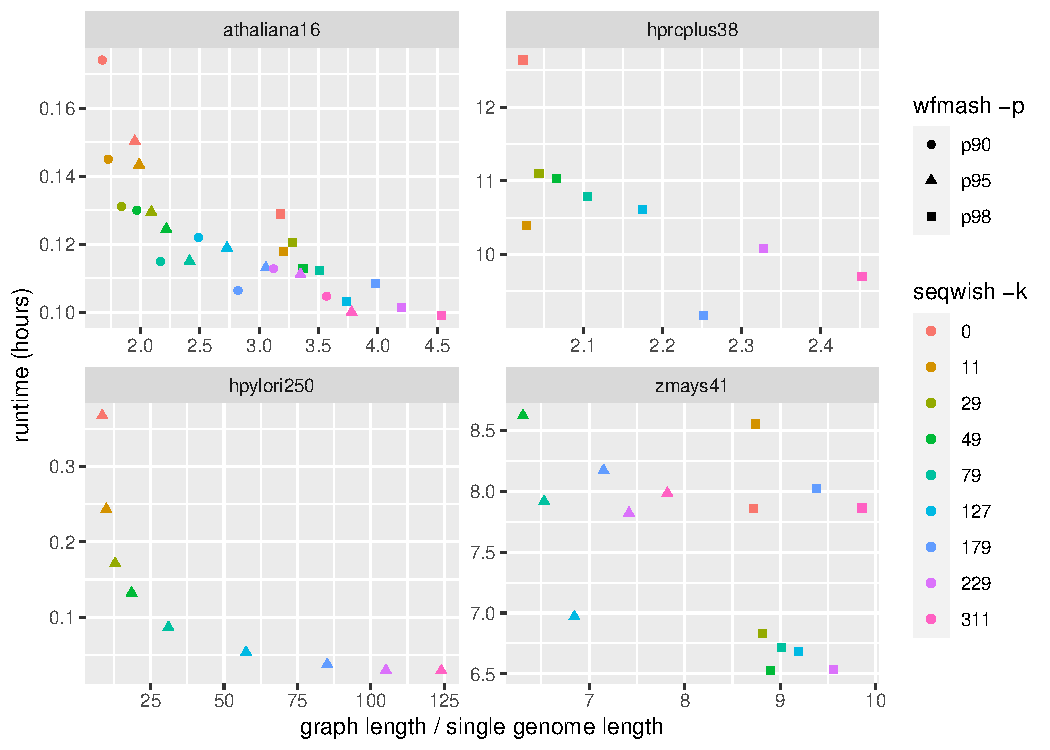
\includegraphics[width=\linewidth, trim=0.4cm 0cm 0.4cm 1cm]{fig_experiment_stats}
   \caption{
     Experimental results from the application of \textit{seqwish} to four different pangenomes.
     Each plot shows the runtime (in hours) versus the average input genome length calculated as the total length of all sequences in the pangenome divided by the number of included haplotypes.
     Multiple minimum identity settings for the mapping (\textit{wfmash -p}) and different minimum match length filter settings (\textit{seqwish -k}) result in a collection of graph builds per pangenome input.
     We compare the runtime in hours with the size of the resulting graphs relative to the average size of an input genome in the particular set.
     Lower limits on pairwise identity result in more compact graphs.
     Similarly, filtering short matches increases graph size relative to not (\textit{seqwish -k}=0, red).
     The other way around, increasing the \textit{seqwish -k} parameter tends to increase the size of the graph.
    }
    \label{fig:experiments}
\end{figure}



\section{Discussion}
\label{sec:discussion}

We have presented a straightforward algorithm to generate a pangenome graph from a collection of genomes and alignments between them.
By exploiting a simple model of this algorithm, we provide computational bounds that give insight into the complexity of the problem.
We then make this approach practical by applying the concept of \textit{match compression}, which reduces the expected computational complexity by a factor proportional to the diversity of input sequences.
Our experimental results demonstrate that we can apply our method to various collections of sequences and alignments.
It easily scales to some of the largest species pangenome construction problems possible using publicly-available, high-quality genome assemblies.
%Although we have focused on the problem of building pangenomes,
\textit{seqwish} is a generic sequence graph inducer of potentially many uses.
We envision that it can serve as a component in diverse sequence analysis and assembly pipelines, and hope that our thorough description of its core algorithm and functionality will enable its reuse by other researchers.

It is also a potentially novel approach.
Despite the existence of many methods for pangenome building, we are not aware of any comparable method which can losslessly convert an all-to-all alignment to a variation graph.
This direct relationship allows users to adjust the shape of the resulting graph by modifying alignment parameters, allowing the design of custom graph construction processes based on domain-specific knowledge and potentially manual curation of assembly alignments.
In contrast to existing methods, which depend on particular structuring of their input \citep{Li:2020,Armstrong:2020}, \textit{seqwish} is unbiased in that as it directly and uniformly represents sequence relationships given on input in the resulting graph.
Although we did not compare with \textit{de Bruijn} graph methods, which are also unbiased in their uniform treatment of input genomes \citep{Minkin_2016,Yu_2021}, we believe such methods are fundamentally different in that because they collapse all exact matches of a given length $k$.
This prevents high-level structuring of patterns of homology and orthology in the resulting graph, and they furthermore cannot be guided by a specific alignment set.

Our presentation is necessarily limited, in order to focus on and describe the unique problem of variation graph induction.
Thus, in this manuscript and our experiments, we have not explored the full problem of \textit{pangenome graph building}, which include both the initial alignment step and downstream processing of the resulting graph.
These topics lie outside of the scope of the presented work, wherein we have focused on a key kernel which is a bottleneck in the pangenome graph construction process.
But, they are important for readers to consider.
Although \textit{seqwish} perfectly represents its input alignments, the problem of generating and filtering an alignment set remains critical, as it determines the structure of the built graph.
And this lossless property does not guarantee that the resulting graph is easy to work with or navigate; in practice, downstream processing is usually required to normalize the graph for many applications.
We will cover these topics in future work.

%However, users of \textit{seqwish} should note that although the graph 
%But, it is important to note that the graphs which it produces are simply raw representations of an underlying alignment set.
%Due to differences in alignments that arise in regions of lower entropy, in practice, it is necessary to normalize generated graphs to simplify the local alignment structures represented in the graph.

\section*{Acknowledgments}

We are grateful to members of the HGSVC and HPRC production teams for their development of resources used in our exposition.
We thank the authors of the pangenome resources made available on GenBank which have made our experiments possible.

\section*{Funding}

We gratefully acknowledge support from NIH/NIDA U01DA047638 (EG) and efforts by Dr. Nicole Soranzo to establish a pangenome research unit at the Human Technopole in Milan, Italy (AG).
\linebreak
\linebreak
\textit{Conflict of Interest}: none declared.

\section*{Data availability}

Code and links to data resources used to build this manuscript and its figures can be found in the paper's public repository: \url{https://github.com/pangenome/seqwish-paper}.

\bibliographystyle{natbib}

\bibliography{document}

\end{document}
